\chapter{ Fundamentação Teórica} \label{cap2}


\corrigir{Neste capítulo serão} apresentados conceitos necessários para o entendimento do trabalho. \commentib{Cite especificamente quais conhecimentos}

\commentib{Creio que antes de falar de identificação, podemos falar um pouco sobre modelos de sistemas dinâmicos. Lá podemos falar de modelos em espaço de estados, função de transferência, EDO's. Daí chegamos em modelos ARX usados na identificação por MQ e modelos em espaço de estados discretos usados em identificação por subespaços.}

\section{Modelos de Sistemas Dinâmicos}
O modelo matemático de um sistema dinâmico é uma forma de descrever uma parte do fenômeno físico que queremos controlar. Nesta seção serão apresentados alguns dos vários modelos matemáticos relacionados ao projeto.
\subsection{Equação Diferencial Ordinária}
Um sistema dinâmico pode ser modelado usando somente a descrição matemática do fenômeno desejado. Usamos como exemplo a modelagem do amortecimento em uma roda de um carro, visto na figura \ref{fig:modeloamortecimento}.

\begin{figure}
	\centering
	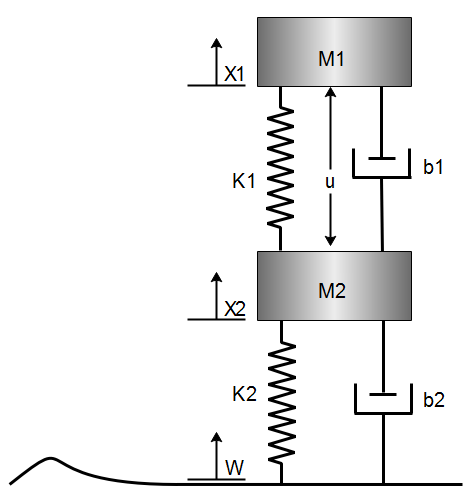
\includegraphics[width=0.5\linewidth]{modelo_amortecimento}
	\caption{Esquema do amortecedor da roda de um carro}
	\label{fig:modeloamortecimento}
\end{figure}

Onde $X_1$ e $X_2$ são a altura das massas $M_1$ e $M_2$, massa do carro e massa da roda, respectivamente. $K_1$ é o efeito elástico do amortecedor e $K_2$ é o efeito elástico da roda. $b_1$ é o efeito amortecedor da suspensão e $b_2$ é o efeito amortecedor da roda.
Esse sistema pode ser modelo em uma E.D.O. (Equação Diferencial Ordinária) usando as leis de Newton, visto nas equações \ref{eq2111} e \ref{eq2112}.

\begin{equation} \label{eq2111}
M_1 \ddot{X}_1=-b_1(\dot{X}_1-\dot{X}_2) -K_1(X_1-X_2)+U
\end{equation}
\begin{equation} \label{eq2112}
M_2 \ddot{X}_2=b_1 (\dot{X}_1 -\dot{X}_2) +K_1(X_1-X_2) +b_2(\dot{W} -\dot{X}_2)+K_1(W-X_2) -U
\end{equation}

\subsection{Funções de Transferência}
A função de transferência é uma equação que descreve o comportamento dinâmico de um sistema relacionando uma entrada com uma saída. Ela é a transformada de Laplace da resposta ao impulso do sistema.

Usando o mesmo sistema da figura \ref{fig:modeloamortecimento} e aproveitando as equações \ref{eq2111} e \ref{eq2112} podemos encontrar as equações de transferência referentes às saídas $X_1$ e $X_2$.

Aplicamos a transformada de Laplace nas equações $X_1$ e $X_2$ para obter:
\begin{equation} \label{eq2121}
(M_1s^2+b_1s+K_1) X_1(s) -(b_1s+K_1) X_2(s)=U(s)
\end{equation}
\begin{equation} \label{eq2122}
-(b_1s+ K_1) X_1(s) +(M_2s^2 + (b_1 + b_2)s +(K_1 + K_2))X_2(s)=(b_2s +K_2) W(s)-U(s)
\end{equation}
Fazendo as devidas manipulações matemáticas chegamos à função de transferência.
\begin{equation}\label{eq2123}
\begin{array}{c}
G_1(s)=\dfrac{X_1(s)-X_2(s)}{W(s)}= \dfrac{(M_1+M_2)s^2+b_2s+K_2} {\Delta}
\\
G_2(s)=\dfrac{X_1(s)-X_2(s)}{W(s)}= \dfrac{-M_1b_2s^3-M_1K_2s^2}{\Delta}
\\
\Delta=(M_1s^2+b_1s+K_1)\cdot (M_2s^2+ (b_1+b_2)s+(K_1+K_2))-(b_1s+K_1)\cdot (b_1s+K_1)
\end{array}
\end{equation}

Com as equações descritas em \ref{eq2123} temos uma equação representando a transferência da entrada para a saída.
\subsection{Espaço de Estados}
A representação em espaço de estados é uma forma mais conveniente para representar sistemas no domínio do tempo quando existe mais de uma entrada ou saída do que a função de transferência. Um modelo linear é representado tipicamente no seguinte formato:
\begin{equation}
\begin{array}{c}
\dot{x}=Ax+Bu\\
y=Cx+Du
\end{array}
\end{equation}
Onde $x \in \Re^n$ é o vetor de estado n-dimensional. $\dot{x}=dx/dt$, $u(t) \in \Re^r$ é o vetor de entradas formado por r funções temporais, $y(t) \in \Re^m$ é o vetor m-dimensional d saídas medidas e, A, B, C e D são matrizes constantes.


Podemos gerar uma representação de espaço de estados a partir da E.D.O. do sistema. Vamos utilizar novamente o sistema da figura \ref{fig:modeloamortecimento}. Definimos primeiramente os estados do vetor x, $x_1=X_1$, $x_2=\dot{X}_1$, $x_3=Y_1$ e $x_4=\dot{Y}_1$. Onde $Y_1=X_1-X_2$, geramos então as matrizes do espaço de estados usando as equações \ref{eq2111} e \ref{eq2112}:
\begin{equation}
\begin{bmatrix}
\dot{X}_1\\
\ddot{X}_1\\
\dot{Y}_1\\
\ddot{Y}_1
\end{bmatrix}
=
\begin{bmatrix}
0 & 1 & 0 & 0\\
\dfrac{-b_1b_2}{M_1M_2} & 0 &\left[ \dfrac {b_1} {M_1} \left( \dfrac {b_1} {M_1} + \dfrac{b_1}{M_2} +\dfrac{b_2}{M_2} \right)- \dfrac{K_1}{M_1}\right] & \dfrac{-b_1}{M_1}\\
\dfrac{b_2}{M_2} & 0 & -\left( \dfrac{b_1}{M_1}+ \dfrac{b_1}{M_2}+ \dfrac{b_2}{M_2} \right) & 1\\
\dfrac{K_2}{M_2} & 0 & -\left( \dfrac{K_1}{M_1} +\dfrac{K_1}{M_2}+ \dfrac{K_2}{M_2} \right) & 0
\end{bmatrix}
\begin{bmatrix}
X_1\\\dot{X}_1 \\Y_1 \\ \dot{Y}_1
\end{bmatrix}
+
\begin{bmatrix}
0 & 0 \\
\dfrac{1}{M_1} & \dfrac{b_1b_2}{M_1M_2}\\
0 & \dfrac{-b_2}{M_2} \\
\left( \dfrac{1}{M_1}+ \dfrac{1}{M_2} \right) & \dfrac{-K_2}{M_2}
\end{bmatrix}
\begin{bmatrix}
U\\W
\end{bmatrix}
\end{equation}
\begin{equation}
Y=
\begin{bmatrix}
0 & 0 & 1 & 0
\end{bmatrix}
\begin{bmatrix}
X_1\\\dot{X}_1\\Y_1\\\dot{Y}_1
\end{bmatrix}
+
\begin{bmatrix}
0 & 0
\end{bmatrix}
\begin{bmatrix}
U \\W
\end{bmatrix}
\end{equation}

\section{Critérios de Estabilidade de sistemas discretos}

O conceito de estabilidade é extremamente importante para a análise de sistemas dinâmicos. Primeiramente definimos  estabilidade de acordo com mudanças nas condições iniciais. Consideremos a equação \ref{eq22}.

\begin{equation} \label{eq22}
x(k+1)=f(x(k),k)
\end{equation}
Sejam $x_0(k)$ e $x(k)$ suas soluções quando as condições inicias são $x_0(k_0)$ e $x(k_0)$. Definimos:


$\bullet$ Estabilidade: A solução $x_0(k)$ é estável se para um dado $\epsilon>0$ existe um $\delta(\epsilon,k_0)$ tal que para todas as soluções com $||x(k_0)-x_0(k_0)||<\delta$ são tais que $||x(k)-x_0(k)||<\delta$ para todos os $k \geqslant k_0$.


$\bullet$ Estabilidade Assintótica: A solução $x_0(k)$ é assintoticamente estável se é estável e um $\delta$ pode ser escolhido tal que  $||x(k_0)-x_0(k_0)||<\delta$ que implica que $||x(k)-x_0(k)||\to\delta$ quando $k \to \infty$.


Existem outros tipos de estabilidade que são de interesse:


$\bullet$Estabilidade BIBO (Bounded-Input Bounded-Output): Um sistema linear invariante no tempo é definido BIBO estável se dado um sinal de entrada limitado ele produz uma saída limitada para cada valor inicial.


Dado que a estabilidade de um sistema é importante para o seu estudo, os métodos para determinar a sua estabilidade são de grande interesse. Os seguintes são alguns dos métodos utilizados para determinar a estabilidade de um sistema:
\begin{itemize}
	\item Cálculo dos autovalores da matriz A da representação de espaços de estado.
	\item Métodos baseados nas propriedades dos polinômios característicos.
	\item O método do lugar das raízes
	\item O método de Lyapunov
\end{itemize}

O cálculo dos autovalores de uma matriz de ordem maior que 2 à mão não é conveniente e em alguns casos é mais fácil calcular a equação característica da forma:
\begin{equation}
A(z)=a_0z^n+a_1z^{n-1}\dots+a_n=0
\end{equation}

E investigar suas raízes utilizando o método do lugar das raízes onde o critério de estabilidade muda para sistemas discretos determinando que para o sistema ser estável todas as raízes devem estar dentro do círculo unitário.

Outro método para determinar a estabilidade de um sistema é o critério de Jury, versão discreta do critério de Routh-Hourwitz. A tabela de Jury é formada da seguinte forma:
\begin{equation}
H(z)=\dfrac{b(z)}{a(z)}=\dfrac{b(z)}{a_0 z^n+a_1 z^{n-1}+\dots+a_n}
\end{equation}
\begin{equation}
\left|
\begin{matrix}
a_0 & a_1& \dots & a_n\\
a_n & a_{n-1}& \dots & a_0\\
b_0 & b_1 & \dots \\
b_{n-1} & b_{n-2} & \dots \\
c_0 & c_1 & \dots \\
\vdots & \vdots
\end{matrix}
\right.
\end{equation}
onde
\begin{equation}
\begin{matrix}
b_0=a_0- \dfrac{a_n}{a_0}a_n\\
b_1=a_1- \dfrac{a_n}{a_0}a_{n-1}\\
\vdots \\
b_k=a_k- \dfrac{a_n}{a_0}a_{n-k}\\
\vdots \\
c_k=b_k- \dfrac{b_{n-1}}{b_0}b_{n-1-k}\\
\end{matrix}
\end{equation}

Com a tabela formada aplicamos o critério de Jury que diz: se $a_0>0$, então todas as raízes estarão dentro do círculo unitário se e somente se todos os termos da primeira coluna das linhas impares forem positivos. Se nenhum elemento da primeira coluna das linhas impares for nulo, o número  de raízes fora do círculo unitário é igual ao número de elementos negativos.

O segundo método de Lyapunov é outra ferramenta útil para determinar a estabilidade de sistemas dinâmicos não lineares. A ideia é introduzir uma função de energia generalizada chamada função de Lyapunov que é zero no ponto de equilíbrio e positiva em outras posições. O equilíbrio será estável se pudermos mostrar que a função de Lyapunov diminui ao longo das trajetórias do sistema.


O primeiro passo é encontrar a função de Lapunov definida como segue:


V(x) é uma função de Lyapunov do sistema
\begin{equation}\label{eqlyap}
x(k+1)=f(x(k)) \qquad f(0)=0
\end{equation}

se:
\begin{enumerate}
	\item V(x) é contínuo em x e V(0)=0
	\item V(x) é definida positiva
	\item $\Delta V(x)=V(f(x))-V(x)$ é definida negativa
\end{enumerate}

Definimos:


$\bullet$Teorema de estabilidade de Lyapunov: A solução $x(k)=0$ é assintoticamente estável se existir uma função de Lyapunov para o sistema da equação \ref{eqlyap}. Se:
\begin{equation}
0<\varphi(||x||)<V(x)
\end{equation}
onde $\varphi(||x||)\to \infty$ quando $||x|| \to \infty$, então a solução é assintoticamente estável para todas as condições iniciais.


A grande dificuldade do teorema de Lyapunov é encontrar uma função de Lyapunov adequada. No entanto, para sistemas lineares como o da equação \ref{eqnsis}, é fácil determinar uma função de Lyapunov quadrática.

\begin{equation} \label{eqnsis}
x_0(k+1)=\Phi x_0(k) \qquad x_0(0)=a_0
\end{equation}

Tomemos $V(x)=x^TP_x$ como candidato para a função de Lyapunov. O incremento de V é dado por:
\begin{equation}
\begin{array}{c}
\Delta V(x)=V(\Phi x)-V(x)=x^T\Phi ^T P \Phi x-x^TPx\\
=x^T(\Phi ^T P \Phi -P)x=-x^TQx
\end{array}
\end{equation}
Para que V seja uma função de Lyapunov é necessário e suficiente que exista uma matriz definida positiva P que satisfaça a equação \ref{eqnLyapunov}.
\begin{equation}\label{eqnLyapunov}
\Phi ^T P \Phi - P= -Q
\end{equation}






\section{Identificação de Sistemas e Estimação de Parâmetros}
A identificação do sistema é o primeiro passo para o seu controle. \commentib{Na verdade, o argumento certo seria dizer que boa parte das técnicas de controle são dependentes de modelos matemáticos, e que modelos podem ser obtidos de diferentes formas (vide Cap. 1 do livro do Aguirre), uma das formas é a identificação, também conhecida como modelagem caixa preta.} \corrigir{Nesta seção serão} tratados conceitos de identificação de sistemas e estimação de parâmetros fundamentais para o entendimento do trabalho.

\subsection{Visão Geral}
A identificação de sistemas e estimação de parâmetros \cortar{se} tratam de métodos e práticas que permitem construir modelos dinâmicos de um sistema \corrigir{ real à partir} de experimentos . Muitas vezes um sistema construído que precisa ser controlado não pode ser modelado devido à limitações matemáticas ou imprecisão na interação dos componentes. \corrigir{ Nestes casos se utiliza} da identificação de sistemas para obter um modelo matemático. A identificação de sistemas se baseia em testar a resposta do sistema à certas entradas e a partir das respostas aproximar o modelo matemático de forma satisfatória. Para identificar sistemas temos métodos determinísticos, que desprezam o ruído presente nos dados, e métodos não paramétricos, que não resultam em um modelo matemático mas em uma representação gráfica da dinâmica do sistema da qual um modelo pode ser extraído. \commentib{Esse último trecho está incorreto ou sem sentido.}


\subsection{Identificação por Mínimos Quadrados}
O método de mínimos quadrados é um dos mais conhecidos e utilizados em várias áreas da ciência e tecnologia. Ele utiliza sistemas de equações com matrizes geradas a partir de testes com os sistemas reais no seguinte formato:

\commentib{Precisamos estabelecer e manter uma notação para diferenciar escalares, vetores, regressores e matrizes.}

\begin{equation}
	\hat{\Theta}=[X^TX]^{-1}X^Ty
\end{equation}
A equação 2.1 é o objetivo da identificação por quadrados mínimos, mas para entender ela precisamos primeiro entender de onde ela vem.
\newline 
Um sistema geralmente é descrito por uma função entrada - saída, em um sistema onde não sabemos a função podemos executar uma série de testes para obtermos um conjunto de valores de entrada e saída da seguinte forma:
\begin{equation}
\begin{array}{c}
y_1=f(x_1) \\
y_2=f(x_2) \\
y_3=f(x_3) \\
\vdots \\
y_N=f(x_N)
\end{array}
\end{equation}
Podemos então tratar esse conjunto como vetores da seguinte forma:
\begin{equation}
y=f(x,\Theta)
\end{equation}
Existem três considerações que devem ser tomadas para avançar o entendimento de mínimos quadrados.
\begin{enumerate}
	\item A função f e o vetor $\theta$ não variam de uma restrição para outra. Todas as restrições são da mesma equação. Em problemas de identificação de sistemas dinâmicos normalmente supõe-se que o sistema seja invariante no tempo e que os sinais medidos sejam estacionários, caso não fossem f e $\theta$ seriam diferentes entre restrições complicando a estimação de um único f e um único $\theta$.
	\item A equação 2.3 pode ser reescrita como
	\begin{equation}
	y=x^T \theta
	\end{equation}
	Implicando que f é linear nos parâmetros. Se f não for linear $\theta$ pode ser estimado por métodos não lineares.
	\item Serão tomadas n restrições de 2.4 a fim de se ter n equações para determinar os n elementos de $\theta$.
\end{enumerate}

Sabendo das considerações as restrições representadas na equação 2.4 podem ser escritas da seguinte forma:

\begin{equation}
\begin{array}{c}
\begin{bmatrix}
y_1 \\ y_2 \\ y_3\\ \vdots \\ y_n
\end{bmatrix}
=
\begin{bmatrix}
x^1_1 & x^2_1 & \dots & x^n_1\\
x^1_2 & x^2_2 & \dots & x^n_2\\
\vdots & \vdots & \ddots& \vdots&\\
x^1_n & x^2_n & \dots & x^n_n\\
\end{bmatrix}
\begin{bmatrix}
\theta_1 \\ \theta_2 \\ \vdots \\ \theta_n
\end{bmatrix}
\\
y=X \theta
\end{array}
\end{equation}
y é uma variável dependente  dos regressores $x_1,... x_n$, também chamados de variáveis independentes. $\theta$ é o vetor de parâmetros a determinar. Desde que X seja não singular é possível determinar o vetor de parâmetros invertendo a matriz:
\begin{equation}
\theta=X^{-1}y
\end{equation}

\commentib{Está faltando no que está descrito acima a descrição de resíduos e de ruídos... Além disso, essa descrição pode ser adequada para estabelecer ligação com equações de diferença e modelos ARX}

\subsection {Filtro de Kalman}
O filtro de Kalman é \melhorar{ um eficiente filtro recursivo que estima o estado de um sistema dinâmico linear a partir de uma série de medições ruidosas}. Ele é utilizado em uma grande variedade de aplicações de engenharia \commentib{Por exemplo?}, e é um tópico especialmente importante para a teoria de sistemas de controle. \commentib{Pq é importante?}
\subsubsection{Visão Geral}
O filtro de Kalman utiliza um modelo dinâmico de um sistema, suas entradas de controle, e \melhorar{ um sistema} de sensores para \melhorar{ gerar uma estimativa das grandezas variáveis} de um sistema \cortar{, seus estados}. Usando um modelo recursivo para obter as estimativas, medidas passadas, ele consegue obter uma estimativa mais fiel ao sistema real do que utilizando somente uma medida. O filtro funciona em duas etapas, uma de propagação, onde se utiliza a estimativa do estado anterior para se obter uma estimativa do estado atual, e uma de assimilação, onde a estimativa do estado atual é combinada com a observação do estado real para se obter um modelo de estimativa mais preciso. \commentib{Quebre linha duas vezes ao invés de usar o comando \texttt{newline}, pois este remove identação.}


Usaremos a nomenclatura de Aguirre, onde $t_1$ é substituído pela iteração atual indicada por k, e o $t_2$ é substituído pela próxima iteração k+1. A notação ($t_1$|$t_1$) é substituída por um sinal '+' para indicar o instante $t_i$ após ter sido incluída a informação em $t_i$. Da mesma forma será utilizado um sinal '-' para indicar a grandeza que se refere ao instante $t_i$ antes de ter sido incluída a informação referente àquele instante. A equação que rege a propagação é a seguinte:
\begin{equation} \label{eq_prop}
\hat{x}^{-}_{k+1}=\Phi_k \hat{x}^+_k+\Gamma_ku_k
\end{equation}

\subsubsection{Etapa de propagação}
Conhecendo a função de densidade de probabilidade de $x_k^+$, indicada por $f_k\sim \mathcal{N}(\bar{x}^+_k, P^+_k)$, deseja-se encontrar a função de densidade de probabilidade de $x^-_{k+1}$. Ou seja, na etapa de propagação deseja-se saber o que acontece à $f_k$ ao ser propagado pela equação \ref{eq_prop}. Assumimos que $f_k$ é gaussiana e portanto $f_-$ também será, deste modo basta determinar $\bar{x}^-_{k+1}$ e $P_-^{k+1}$ contidos em $f_- \sim \mathcal{N}(\bar{x}^-_{k+1},P^-_{k+1})$ para caracterizar $f_-$.


Seguindo o raciocínio de \commentib{Essa citação está inadequada} Aguirre encontramos:
\begin{equation}
\bar{x}^-_{k+1}=\Phi_k\bar{x}^+_k+\Gamma_ku_k
\end{equation}
\begin{equation}
P^-_{k+1}=\Phi_kP^+_k\Phi^T_k+\Upsilon_kQ_k\Upsilon^T_k
\end{equation}

A equação mostra que ao longo da etapa de propagação a incerteza aumenta devido à presença de ruído no modelo dinâmico usado.

\subsubsection{Etapa de assimilação}
Vimos que na etapa de propagação o vetor de estado $x^+_k$ é propagado para a próxima iteração resultando em $x^-_{k+1}$. A segunda etapa, a de assimilação, ocorre com a chegada de nova informação na iteração k+1. O objetivo é a determinação de $f_+ \sim \mathcal{N} (\bar{x}^+_{k+1},P^+_{k+1})$ a partir de $f_-$ e da medição na iteração $y_{k+1}$. De forma semelhante à etapa de propagação, devemos encontrar $\bar{x}^+_{k+1}$ e $P^+_{k+1}$. Após os devidos passos encontramos:
\begin{equation}
\bar{\mathbf{x}}^+_{k+1}=\bar{\mathbf{x}}^-_{k+1}+K_{k+1}[\mathbf{y}_{k+1}-H_{k+1} \bar{\mathbf{x}} ^-_{k+1}]
\end{equation}
\begin{equation}
P^+_{k+1}=P^-_{k+1}-K_{k+1} H_{k+1} P^-_{k+1}
\end{equation}
\begin{equation}
K_{k+1}=P^-_{k+1} H^T_{k+1}[H_{k+1} P^-_{k+1} H^T_{k+1}+R_{k+1}]^-1
\end{equation}

Com estas equações completamos o conjunto de equações necessárias para entender o filtro de Kalman.
\subsection {Identificação por Subespaços}



% Fim Capítulo















